%======================================================================
\section{Systems, data and ground truth}
\label{sec:systems}
%======================================================================

We use three periodic, scalar, spatiotemporally chaotic systems of
increasing difficulty: the one-dimensional Kuramoto--Sivashinsky (KS)
equation, its two-dimensional isotropic generalization, and
two-dimensional Kolmogorov flow with linear drag. All three are
integrated in Fourier space with a fourth-order exponential time-differencing
Runge--Kutta scheme (ETDRK4), with the coefficients evaluated by the
contour-integral method of \citet{kassam2005} (32 points), in double
precision on the CPU. Table~\ref{tab:systems} collects the parameters,
Table~\ref{tab:truth} the ground-truth Kaplan--Yorke dimensions, and
Appendix~\ref{app:groundtruth} the full protocol and the solver
validation. Figure~\ref{fig:systems} shows each system on the domain its
models are trained on.

\begin{figure*}[htbp]
\centering
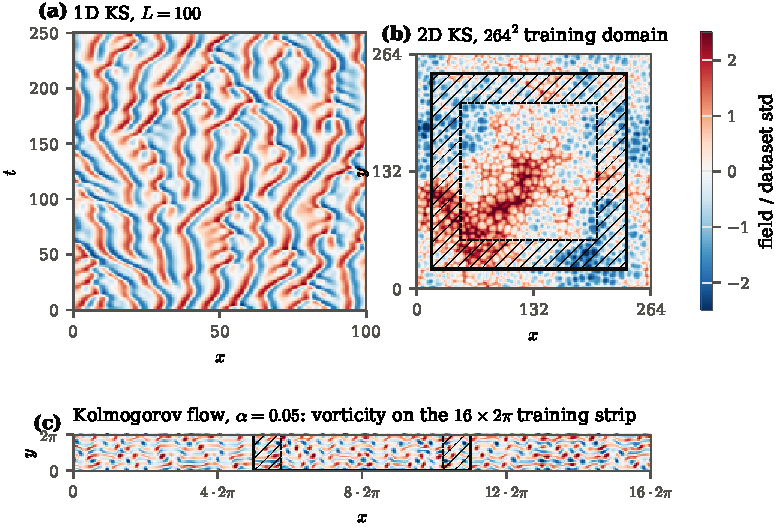
\includegraphics{figures/fig02_systems.pdf}
\caption{The three systems on their training domains, standardized by
the training standard deviation. (a) 1D KS at $L=100$: 250 time units
of one training trajectory. (b) 2D KS: one snapshot on the $264^2$
periodic domain whose windows train the 2D KS model; the outlined square
is one $40\times40$-site training window, its forced halo (six sites)
hatched and its free interior inside the dashed line. (c) Kolmogorov flow
at $\alpha=0.05$: vorticity on the $16\times2\pi$ by $2\pi$ training strip,
with one 48-site window spanning the full height and its six-site halo in
$x$. Cells of a fixed size fill the 1D and 2D KS domains, and the
Kolmogorov vortices are organized by the forcing at wavenumber 4 in
$y$; in each case the domain holds many independent copies of the local
dynamics, which is what window training samples.}
\label{fig:systems}
\end{figure*}

%----------------------------------------------------------------------
\subsection{One-dimensional Kuramoto--Sivashinsky}
\label{sec:ks1d}
%----------------------------------------------------------------------

The KS equation \citep{kuramoto1976,sivashinsky1977},
\begin{equation}
  u_t + u u_x + u_{xx} + u_{xxxx} = 0, \qquad x\in[0,L),
  \label{eq:ks1d}
\end{equation}
has a linear growth rate $k^2-k^4$ that is positive for $|k|<1$ and
largest at $k=1/\sqrt2$, which sets a pattern wavelength of
$2\sqrt2\,\pi\approx8.9$. For $L$ large compared with this length the
dynamics are extensively chaotic, with $\DKY\approx0.226L$ minus a
small offset \citep{manneville1985,edson2019}. We train at $L=100$ on a
grid of $256$ points ($\Delta x = 0.39$), with solver step $0.05$ and
snapshot interval $\Delta t=1.0$. The training set has 60 independent
trajectories (50 training, 10 validation) of 250 time units each, after
a spin-up of 500 time units.

Ground truth is computed at $\Delta x = 100/1024$, four times finer than
the training grid, to keep the solver error well below the model error,
with averaging windows of 1200--2000 time units (100 or more Lyapunov
times for $L\ge50$). At $L=100$ the reference value is $\DKY=22.5$,
inside the range $[21,24]$ reported in the literature, with
$\lambda_1=0.090$ and 12 positive exponents; \citet{edson2019} give
$\DKY\approx0.226L-0.16$ for $L\gtrsim80$, i.e.\ $22.4$. At $L=22$ our
solver gives $\DKY=5.26$ and $\lambda_1=0.049$, against $5.20$ and $0.043$
from \citet{edson2019} and a leading exponent of $0.048$ from
\citet{cvitanovic2010}. The transfer sizes $L=25,50,200,400$ give the
densities in Table~\ref{tab:truth}: $\DKY/L$ lies between $0.224$ and
$0.226$ for every $L\ge50$, while at $L=25$, close to the onset of
chaos, $\lambda_1\approx0.001$ and the density falls to about $0.07$.

%----------------------------------------------------------------------
\subsection{Two-dimensional Kuramoto--Sivashinsky}
\label{sec:ks2d}
%----------------------------------------------------------------------

The isotropic 2D generalization,
\begin{equation}
  u_t + \nabla^2 u + \nabla^4 u + \tfrac12|\nabla u|^2 = 0,
  \qquad (x,y)\in[0,L)^2,
  \label{eq:ks2d}
\end{equation}
has the same linear operator, now unstable on the ring $|\bm k|<1$
\citep{kalogirou2015}. Unlike the 1D equation, its nonlinearity is not a
total derivative and drives the spatial mean of $u$. The mean carries
no dynamical information (only gradients of $u$ enter the right-hand
side), so we project the $\bm k=0$ mode out after every step, in the
base trajectory and in every tangent vector. All runs use solver step
$0.02$, snapshot interval $\Delta t=0.1$ and grid spacing
$\Delta x = 0.344$ ($128$ points at $L=44$).

The training data are four trajectories (plus one for validation) of
25 time units on a single periodic domain of side $264=6\times44$
($768^2$ points), after a spin-up of 200 time units. Models are crop-trained
on this domain (Sec.~\ref{sec:crop_training}) and evaluated on square
periodic boxes of side $44$, $66$ and $88$. Ground truth exists at $44^2$
(three runs, $\DKY=80.7$--$83.6$, mean $82.0$, 42--44 positive exponents)
and $66^2$ (two runs, $185.6$ and $192.5$, mean $189.1$, 93--101 positive
exponents). The mean densities, $0.0424$ and $0.0434$ per unit area,
differ by $2.5\%$, inside the spread of the individual runs; we did not
compute a truth at $88^2$, where the expected dimension (about 330) would
need more than 500 tangent directions.

%----------------------------------------------------------------------
\subsection{Kolmogorov flow with linear drag}
\label{sec:kolmogorov}
%----------------------------------------------------------------------

Two-dimensional incompressible flow in vorticity form,
\begin{equation}
\begin{gathered}
  \omega_t + \bm u\cdot\nabla\omega = \nu\nabla^2\omega - \alpha\,\omega + f(y),\\
  \bm u = (\psi_y,-\psi_x),\qquad \nabla^2\psi=-\omega,
\end{gathered}
  \label{eq:kolmogorov}
\end{equation}
on $[0,L_x)\times[0,2\pi)$, with forcing
$f(y) = -(\nu n^2+\alpha)\,n\cos(ny)$. This forcing makes
$\bm u = (\sin ny, 0)$ an exact steady solution for every $\alpha$, which
gives an exact test of the solver (Appendix~\ref{app:groundtruth}).
We use $n=4$ and $\nu=0.01$, and three drag coefficients
$\alpha\in\{0.025,0.05,0.1\}$. We quote a Reynolds number
$Re=\sqrt{f_0}/\nu$ built from the velocity forcing amplitude
$f_0=\nu n^2+\alpha$ on a $2\pi$ box; this is the definition of
\citet{kolmogorovregimes2026} applied to our forcing, and coincides with
theirs for $\alpha=0$ (their flows have no drag). Our three drags give
$Re\approx43$, $46$ and $51$.

The drag is what makes the flow usable for domain transfer. Without it,
the two-dimensional inverse energy cascade accumulates energy at the
largest scale the box allows
\citep{kraichnan1967,smithyakhot1993,boffettaecke2012}, so the
statistics depend on the domain size and the dimension cannot be
extensive. With drag, the dimension per $2\pi\times2\pi$ box changes
by at most about $20\%$ between one and three boxes at every $\alpha$ we
use (Table~\ref{tab:truth}), comparable to the uncertainty of the
single-run truths (Sec.~\ref{sec:truth_uncertainty}); without drag the
flow condenses into a domain-scale mean state.

The forcing singles out $y$: the equation is translation-invariant in
$x$ and invariant in $y$ only under shifts by the forcing period $2\pi/n$.
We therefore keep the height fixed at $2\pi$ and grow the domain in $x$
only, to $2\times$ and $3\times$ the square box. Kolmogorov results are
statements about widening the channel, not about growing its area in
both directions; the 2D KS results are the isotropic test. All runs use
grid spacing $2\pi/128$, solver step $0.01$ and snapshot interval
$\Delta t=0.2$. Training data come from a domain of width $16\times2\pi$
($2048\times128$ points), four training and one validation trajectory of
40 time units per drag value, after a spin-up of 100 time units.

%----------------------------------------------------------------------
\subsection{How precise is the ground truth?}
\label{sec:truth_uncertainty}
%----------------------------------------------------------------------

Every comparison in this paper is between a model's $\DKY$ and a
finite-time estimate of the true $\DKY$ from one or a few initial
conditions. The precision of that estimate differs greatly between the
systems, and it limits what can be claimed.

\para{1D KS.} Windows of 1200--2000 time units span 100 or more
Lyapunov times for $L\ge50$. Runs that differ only at round-off level
(the thread count of the FFT) follow different chaotic trajectories, and
we use them as independent finite-time samples: at $L\ge50$ two or
three such runs agree to within $0.1$--$2\%$, and the mean densities
agree to within $1\%$ across a factor of 8 in $L$. We treat the 1D
truths as accurate to about one percent.

\para{Kolmogorov flow.} Lyapunov times are 6--16 time units, so a
40-unit window covers only 2--6 of them. We measured how much this
matters. For five truth runs averaged over 120 time units, we recorded
the running estimate of $\DKY$ every 20 units
(Fig.~\ref{fig:truth_convergence} in Appendix~\ref{app:groundtruth}).
The running value at $t=40$ is what a 40-unit run from the same
initial condition returns; for the three $\alpha=0.05$ runs, which
continue the trajectories of earlier 40-unit truth runs, it reproduces
those truths to within $0.2\%$ (for example $38.68$ and $53.89$).
Relative to the 120-unit value, the 40-unit value was off by $-17\%$ to
$+23\%$ and high in five of seven runs, by $9\%$ on average;
over the last 20 units the running estimates still moved by up to
$5\%$. Independent initial conditions at a fixed size and window
differ by $3.7\%$ at $\alpha=0.1$, $2\times$, by $11.3\%$ at $\alpha=0.1$,
$3\times$, by $12.4\%$ at
$\alpha=0.05$, $2\times$, and by $9\%$ at $\alpha=0.05$, $1\times$.

\para{2D KS.} The truths use 40-unit windows (about 7 Lyapunov times).
Independent initial conditions give $80.7$, $81.8$ and $83.6$ at $44^2$
($\pm1.8\%$) and $185.6$ and $192.5$ at $66^2$ ($\pm1.8\%$), and the running
estimates still move by $3$--$5\%$ over the last 20 time units. We treat
the 2D KS truths as uncertain at the level of a few percent.

\para{Convention used in this paper.} Where several truth runs exist
for one configuration we use their mean (Table~\ref{tab:truth}): two or
three runs for every 1D size, three at $44^2$ and two at $66^2$ for 2D KS,
and three at $\alpha=0.05$, $2\times$ and at $\alpha=0.1$, $2\times$ and
$3\times$ for Kolmogorov flow.
At $\alpha=0.05$, $1\times$, the three 120-unit truths start from the
same initial conditions as the model evaluations, and we score each
model run against its matched truth; since a model's own single-run
estimate at this size scatters strongly (Sec.~\ref{sec:evaluation};
Fig.~\ref{fig:appendix_panels}(a)), this removes truth-side noise only. The remaining Kolmogorov sizes
($\alpha=0.1$, $1\times$; $\alpha=0.05$, $3\times$; all three sizes at
$\alpha=0.025$) rest on a single run. We report the Kolmogorov results as scaling of $\DKY$ with
domain size, with the spread above as the truth's error bar, and treat
differences between a model and a single 40-unit truth of 10--15\% as
within the uncertainty of the reference rather than as model error. The
1D results carry no such caveat.

%----------------------------------------------------------------------
\begin{table*}[htbp]
\caption{Systems and data. $\Delta x$ is the grid spacing,
$\Delta t$ the snapshot interval seen by the model, ``train domain'' the
domain from which training data (crops, for 2D) are drawn, and ``eval''
the domain sizes at which models are compared with ground truth.}
\label{tab:systems}
\begin{ruledtabular}
\begin{tabular}{lcccc}
system & $\Delta x$ & $\Delta t$ & train domain (trajectories) & eval sizes \\
\hline
1D KS & $0.39$ & $1.0$ & $L=100$ (50+10) & $L=25,\,50,\,100,\,200,\,400$ \\
2D KS & $0.344$ & $0.1$ & $264\times264$ (4+1) & $44^2,\,66^2,\,88^2$ \\
Kolmogorov$^{a}$ & $2\pi/128$ & $0.2$ & $32\pi\times2\pi$ (4+1) & $L_x=2\pi,4\pi,6\pi$; $L_y=2\pi$ \\
\end{tabular}
\end{ruledtabular}
\footnotesize{$^{a}$\,$n=4$, $\nu=0.01$, $\alpha\in\{0.025,0.05,0.1\}$.}
\end{table*}

\begin{table*}[htbp]
\caption{Ground-truth Kaplan--Yorke dimensions. $T$ is the averaging
window in time units; the number in parentheses is the number of
independent runs (1D: distinct finite-time realizations, see
Appendix~\ref{app:groundtruth}). Density is $\DKY$ per unit length (1D KS), per unit area
(2D KS), or per $2\pi\times2\pi$ box (Kolm., Kolmogorov flow, here and in
every table). Values in bold are the
references used in the paper (means where several runs exist).}
\label{tab:truth}
\widetabular{llcccl}{
system & size & $\DKY$ & density & $T$ (runs) & note \\
\hline
\tabinput{tables/tab02_truth}}
\end{table*}
